\chapter{Evaluation}
\label{chap:eval}

In this chapter, we apply EzQL to some real-world event processing
problems and discuss how does it compare to solutions written in other languages.

\section{The ``too muggy query''}

This query was first introduced in section
\ref{sec:defective-products}, where we also presented and discussed a
solution implemented in Coral8 CCL. The equivalent program in EzQL is
as follows:

\begin{lstlisting}
tempReadings = stream of { roomId:int, temperature:int }
entries = stream of { roomId:int, productId:int }

entity Room =
  createFrom(tempReadings, :roomId)

entity Product =
  createFrom (entries, :productId)
  belongsTo :room
  member this.temperature = this.room.temperature

defective =
  from p in Product.all
  where (p.temperature > 25).howLong() >= 10 min
\end{lstlisting}

This example uses only operators shown in chapter \ref{chap:ezql} and
thus, should not be difficult to understand. We begin by declaring the
input streams, then we define the \verb=Room= and \verb=Product=
entities, and finally, we declare the ``too muggy'' query that solves
the problem.

One of the issues with the solution presented in section
\ref{sec:defective-products} is that it doesn't solve the entire
problem, because it ignores humidity. The following listing extends
the example above to support humidity:

\begin{lstlisting}
# input streams
tempReadings = stream of { roomId:int, temperature:int }
humReadings = stream of { roomId:int, humidity:int }
entries = stream of { roomId:int, productId:int }

tempsAndHums = merge(tempReadings, humReadings, :roomId)

# define the entities
entity Room =
  createFrom(tempsAndHums, :roomId)

entity Product =
  createFrom (entries, :productId)
  belongsTo :room
  member this.temperature = this.room.temperature
  member this.humidity    = this.room.humidity

# which products are defective?
defective =
  from p in Product.all
  where (p.temperature > 25 and p.humidity > 80).howLong() >= 10 min
\end{lstlisting}

We begin by declaring a new stream -- \verb=humReadings= --, which is
merged with \verb=tempReadings=. \verb=merge= is a simple operator
that receives events from two streams and joins them into one. Every
time an event arrives on any input stream, it is sent to the single,
output stream. However, if two events arrive at the same time on both
streams, \verb=merge= will try to join them if they share a common
field -- \verb=roomId= in this example. In other words, if
\verb=tempReadings= receives these events:

\begin{tabular}{ |l|l|c| }
  \hline
  \verb=timestamp= & \verb=roomId= & \verb=temperature= \\
  \hline
  11:00:00 am & \verb="A"= & 20 \\
  11:01:00 am & \verb="B"= & 29 \\
  \hline
\end{tabular}

and \verb=humReadings= receives these:

\begin{tabular}{ |l|l|c| }
  \hline
  \verb=timestamp= & \verb=roomId= & \verb=humidity= \\
  \hline
  11:00:00 am & \verb="C"= & 67 \\
  11:01:00 am & \verb="B"= & 73 \\
  11:02:00 am & \verb="A"= & 75 \\
  \hline
\end{tabular}

then \verb=merge(tempReadings, humReadings, :roomId)= will result in:

\begin{tabular}{ |l|l|c|c| }
  \hline
  \verb=timestamp= & \verb=roomId= & \verb=temperature= & \verb=humidity=\\
  \hline
  11:00:00 am & \verb="A"= & 20 & null \\
  11:00:00 am & \verb="C"= & null & 67 \\
  11:01:00 am & \verb="B"= & 29 & 73 \\
  11:02:00 am & \verb="A"= & null & 75 \\
  \hline
\end{tabular}

When the events are not merged -- either because there was only one
event or the events didn't match --, \verb=merge= fills the unknown
fields with \verb=null=. In EzQL, most operators on continuous values
ignore \verb=null=, which means that, for example, the temperature of
room A remains at 20 degrees at 11:02:00 am. Also, note that
\verb=merge= may put two different events with the same timestamp into
the same stream, which means EzQL demands support for simultaneous
events.

We use the result of merging both streams to instantiate the
\verb=Room= entity. Thus, every \verb=Room= instance will
automatically be equipped with \verb=temperature= and \verb=humidity=
field. We them use this last field to define the \verb=Product='s
humidity, much like we had done previously with the temperature. At
last, in the final line, we update the condition to take humidity into
account.

\section{Linear road benchmark}

The Linear Road benchmark \cite{lrb} was introduced as a first attempt
at producing a realistic benchmark for ESP engines. In \cite{cql}, the
creators of CQL implemented a simplified version to introduce their
language and discuss its semantics. This makes the linear road
benchmark of particular importance, because it allows us to compare
EzQL with CQL, using an example that, presumably, CQL handles well.

The benchmark itself models a road traffic management scenario with a
number of highways where the cost of traveling is calculated in
real-time and is dependent on the traffic conditions. Intuitively, a
costumer pays more if he chooses to drive by a congested segment,
because he is contributing for the increase in traffic inside that
segment. Hopefully, the common goal to pay less somehow drives
costumers to regulate traffic in a way that is beneficial for
everyone.

\begin{figure}[t]
  \centering
  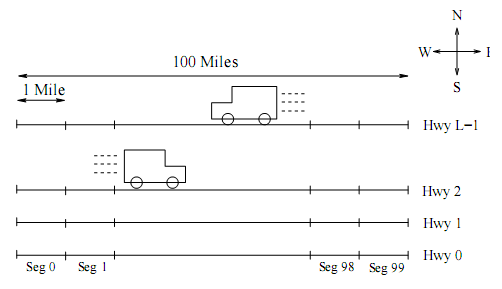
\includegraphics[width=0.6\textwidth]{lrb.png}
\caption{The linear-road highway system. Image taken from \cite{cql}}
\end{figure}


To simplify, we assume the highways run from east to west. All
vehicles report their position and velocity every 30 seconds to a base
station. The position is specified using three attributes: the highway
number, the direction (east or west) and the distance the vehicle is
from the western endpoint of the highway. A base station aggregates
this data to calculate the toll for each segment. For non-congested
segments, the toll is 0. For congested segments, on the other hand,
the toll is calculated using the formula \(basetoll * (numvehicles -
150)^2\), where \(baseToll\) is a constant parameter and
\(numvehicles\) is the number of vehicles currently in the
segment. Furthermore, a segment is considered to be congested if the
average speed of all vehicles in that segment over the last 5 minutes
is less than 40 mph. Finally, we assume that highways are 100 miles
long and are divided into one hundred 1-mile segments. Thus, the current
segment of a vehicle is defined by the triple (highway, direction,
xPos/1760). The input for this problem is a single stream with the
position and speed reports for all vehicles. We use this stream to
find an answer to our main problem: how much does each costumer pay in
the end?

The solution in CQL, taken from \cite{cql}, is transcribed in appendix
\ref{sec:lrb-cql}. The algorithm consists in applying successive
operations to the input stream to produce a few derived streams and
relations, which are then combined to compute the answer. Figure
\ref{fig:lrb-cql} shows how these derived streams and relations
interact with each other.

\begin{figure} \centering
  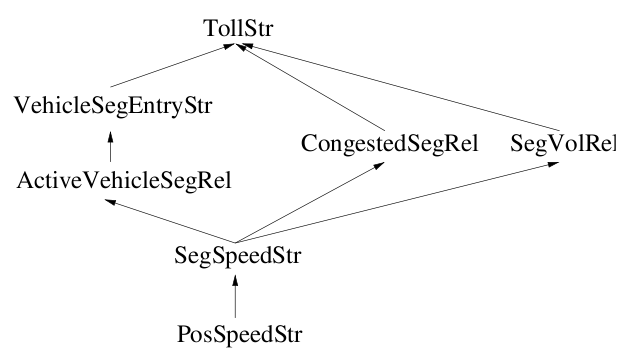
\includegraphics[width=0.5\textwidth]{lrb-cql.png}
  \caption{Derived streams and relations in the solution to the linear
    road benchmark. Image taken from \cite{cql}.}
  \label{fig:lrb-cql}
\end{figure}


The six queries are not difficult to understand by
themselves. However, the simple fact that the authors had to create a
diagram to explain their solution should raise an alarm. All these
temporary streams and relations show a symptom that we already
discussed in section \ref{sec:defective-products}: the only way to
manage complexity using existing languages is through the creation of
a large number of intermediary streams and windows, which are coupled
with each other in ways that violate most best-practices. A second
problem with this solution is related to time management. For example,
the last query outputs the toll for each vehicle that enters a
segment. We copy it here for easier reference:

\lstset{
  language=CCL,
  columns=fullflexible,
  basicstyle=\tt,
  keywordstyle=[1]\bf,
  keywordstyle=[2]\it,
}

\begin{lstlisting}
# Query 6: TollStr(vehicleId,toll)

Select Rstream(E.vehicleId,
               basetoll * (V.numVehicles - 150)
                        * (V.numVehicles - 150) as toll)
From VehicleSegEntryStr [Now] as E,
     CongestedSegRel as C, SegVolRel as V
Where E.segNo = C.segNo and C.segNo = V.segNo and
      E.dir = C.dir and C.dir = V.dir and
      E.hwy = C.hwy and C.hwy = V.hwy
\end{lstlisting}

\lstset{
  language=EzQL,
  columns=fullflexible,
  basicstyle=\tt,
  keywordstyle=[1]\bf,
  keywordstyle=[2]\it,
}

To control precisely when this query should be executed, an inner join
between three entities is performed, one of which is a stream that
signals the entry of a vehicle in a new segment. However, this is not
immediately obvious. We believe that developers should not need to
worry with the exact time a query is executed: that is a low level
detail that should be abstracted by the system. However, if the
problem requires such fine-grained control, there must be a better way
to do it than joining streams. A third and final problem with this
example pertains to the way the toll is calculated. In the last query,
the toll is calculated for each vehicle. However, this does not make
sense from a modeling point of view: the toll is an attribute of the
segment, not of the vehicle. This could probably be easily changed.
But the point is: CQL does not provide any means to enforce an
accurate modeling of the problem at hand, which reinforces our idea
that all these streams are only temporary and won't be used
extensively as a building-block for other queries.

The equivalent solution in EzQL is presented below:

\begin{lstlisting}
posSpeedStr = stream of { vehicleId:int, speed:int, hwy:int,
                             dir:bool, pos:int }

baseToll = 100 # any value will do

# Convert x coordinates to segment numbers
segSpeedStr =
  from ev in posSpeedStr
  select { vehicleId = ev.vehicleId, speed = ev.speed,
           segmentId = (ev.hwy, ev.dir, ev.pos / 1760) }

entity Segment =
  createFrom(segSpeedStr, :segmentId)
  hasMany :vehicles

  # A segment is congested if the speed average reported over the
  # last 5 minutes is less than 40 mph
  member this.isCongested =
    let avg5mins = this.events[5 min].avg(:speed)
    if avg5mins.null?
      then false
      else avg5mins < 40

  # The toll for this segment
  member this.toll =
    if this.isCongested
      then baseToll * (this.vehicles.count() - 150) ^ 2
      else 0

entity Vehicle =
  createFrom(segSpeedStr, :vehicleId)
  belongsTo :segment

  member this.amount = 0
    when this.segmentId.changes() -> this.amount + this.segment.toll


# amount per vehicle
amountPerVehicle =
  from v in Vehicle.all
  select v.amount
\end{lstlisting}

We begin by converting the position coordinates sent by the vehicles
into segment numbers. Note that the \verb=segmentId= field is a triple
containing the highway number, the direction and the segment number.
Then, we use the resulting stream to define the \verb=Segment= and
\verb=Vehicle= entities. We then define the \verb=isCongested= member,
that checks if a \verb=Segment= is congested. It does so by getting
the average speed over the last 5 minutes in the \verb=this.events=
member. As explained in chapter \ref{chap:ezql}, \verb=events= is a
stream created automatically by \verb=createFrom= that contains all
the events related to this segment. If there were no cars in this
segment during that interval, the segment is not congested for
sure. Otherwise, it is congested only if the average is below 40
mph. We then proceed by calculating the current toll for each segment,
using the formula given above. For the \verb=Vehicle= entity we define
the single attribute \verb=amount= that starts at 0, but is
incremented by the current segment's toll every time the vehicle
changes to a different segment. Finally, the last few lines declare a
query that obtains, for all vehicles, the amount they have to pay.

How does our solution compare to the one written in CQL? For starters,
instead of defining several streams and relations, we model the
scenario by declaring two queries and defining two entities. These
entities group several members together that may be seen as attributes
of their instances. This is an important difference, because when the
developer adds a new member to an entity, he is somehow forced to
think ``does this make sense?''  or ``will this interfere with the
work of my coworkers?''. Intermediate streams, on the other hand, are
used in isolation, as local variables in a procedure. Hence, most
developers don't really care if these streams could be reused or if
they model the scenario accurately, which means they will become
forgotten after a couple usages.

Another important difference is that we use when blocks to specify
\emph{when} the amount to pay be should updated. In our opinion, this
is clearer than joining streams and windows.

% TODO: Say that it is shorter (but is it?)

%\begin{figure}[htbp]
%  \centering
%  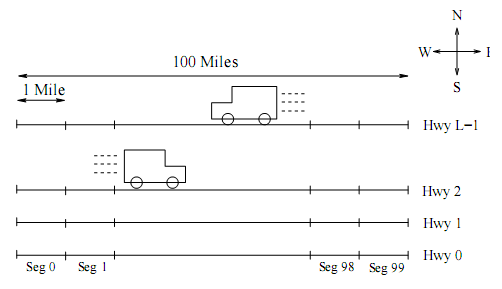
\includegraphics[width=\textwidth]{lrb.png}
%  \caption{Dependency graph for the Linear Road benchmark.}
%  \label{fig:eventflow-sample}
%\end{figure}



\section{Stock data analysis}

In this section we implement a few common financial market analysis
indicators that may be used to support the trading decision
process. The reader is advised not to adventure himself into this
hostile market armed solely with these primitive algorithms.

\subsection{MACD}

MACD \cite{macd-book} -- or Moving Average Convergence/Divergence --,
is a financial market indicator created by Gerald Appel that may be
used to predict the right time to sell or buy stocks from some
company, using only the past evolution in their prices. Its
calculation is very simple:

\begin{enumerate}
\item First, we calculate the exponential moving average (EMA) of the
  prices over the last 12 and 26 days (these numbers are only
  recommendations) and subtract them. This gives us the \emph{MACD};
\item Then, we obtain another exponential moving average over the MACD
  itself, regarding the last 9 days. This gives us the \emph{signal}.
\end{enumerate}

Figure \ref{fig:macd} shows all these values plotted against the price
of some company's stocks. We can now subtract the MACD by the signal
to find out, using a very primitive algorithm, if we should be buying
or selling stocks from that company. If the MACD becomes greater than
the signal, we should buy. Otherwise, if the MACD goes below the
signal, we should sell.

\begin{figure}[t]
  \centering
  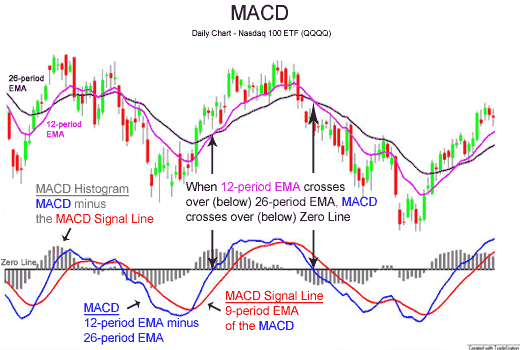
\includegraphics[width=0.6\textwidth]{macd.png}
  \caption{Sample plot showing the evolution of some stocks, as well
    as both 12 and 26 EMAs (in pink and black), the MACD (in blue) and
    the signal line (in red). Image copied from \cite{macd-plot:www}.}
  \label{fig:macd}
\end{figure}

StreamBase, one of the leading event processing products in the
market, comes with a sample project that calculates the MACD, which
should make for an interesting comparison. The code, copied as is from
the sample, is shown in section \ref{sec:macd}. Our solution is as
follows:

\pagebreak
\begin{lstlisting}
stocks = stream of { timestamp:int, symbol:string, value:float }

# Produces an event every day, at midnight.
midnight =
  from ev in ticks
  where ev.timestamp % 86400 == 0

entity Company =
  createFrom (stocks, :symbol)

  # Yesterday's final value
  member this.yesterday = 0.0
    when midnight -> this.value # value is created by createFrom

  member this.trend =
    let macd = ema(this.yesterday, 12) - ema(this.yesterday, 26)
    let signal = ema(macd, 9)
    macd - signal

  # Should we buy or sell stocks from this company?
  member this.buy = this.trend > 0
  member this.sell = this.trend < 0


toBuy =
  from c in Company.all
  where c.buy

when ev in toBuy.values().added() ->
  print("You should buy stocks from " + ev.value.symbol)
\end{lstlisting}

This snippet begins with the declaration of the \verb=midnight=
stream, using a variable that has not yet been introduced --
\verb=ticks=. This is a predefined stream that emits an event once per
second. \verb=midnight= filters all these events except one per
day. Thus, if the program begins execution at midnight, the stream
\verb=midnight= will actually output an event every day, at midnight,
thus notifying its users the day has changed. Naturally, it is not
realistic to demand this restriction in a real-world application, but
in this example it will do, as it is more or less orthogonal to the
calculation of the MACD.

Next, we define a \verb=Company= entity that has four attributes. The
first -- \verb=yesterday= --, contains yesterday's last price. Note
that this value is updated once per day. Thus, if we open a window
over it, we may get the closing prices of the previous days. The
second member -- \verb=trend= --, calculates the difference between
the MACD and the signal lines using the closing prices of the last few
days. Finally, \verb=buy= and \verb=sell= are simply the indicators we
want to monitor in order to make decisions.

At last, we declare a dictionary to contain all companies where the
\verb=buy= signal is enabled. In the final two lines, we monitor which
companies are added into this dictionary. These are the companies
where the MACD has just crossed the signal and, according to the
algorithm above, this is when we should be buying their stocks. As
discussed previously, the \verb=values()= operator returns a list with
the values in a dictionary. Using this list, we may then apply the
\verb=added()= operator to find out when a new entry is added into the
dictionary. There is also a corresponding \verb=expired()= operator that
signals the removal of an entry.

The example above uses the \verb=ema()= function to calculate the
exponential moving average. This is an user-defined aggregator
implemented in EzQL as follows:

\begin{lstlisting}
enum EmaState =
  | Init of { count:int, sum:float }
  | Normal of float

def ema(data, n) =
  let alpha = 2 / (n + 1.0)
  let result = Init ({ cnt = 0, sum = 0.0 })
    when data.changes() ->
      match result with
        | Init s ->
            if s.cnt < 2
              then Init ({ cnt = s.cnt + 1, sum = s.sum + data })
              else Normal ((s.sum + data) / (s.cnt + 1))
        | Normal f -> Normal (alpha * data + (1 - alpha) * f)

  match result with
    | Init s -> if s.cnt == 0 then 0 else s.sum / s.cnt
    | Normal f -> f
\end{lstlisting}

This code is complicated by the initialization: when there is no
history we can't calculate an EMA. Instead, we begin by calculating a
regular arithmetic mean. After 3 values are in, we switch to the real
EMA. This solution differentiates these two phases into two states
defined in \verb=EmaState=: \verb=Init= -- which contains a count and
a sum needed to calculate the mean -- and \verb=Normal= -- which
contains only the EMA's value. \verb=result=, which keeps this state,
begins in the \verb=Init= state with both \verb=sum= and \verb=cnt=
initialized at 0. When the value changes, if this is only the first or
second update, it updates the \verb=count= and \verb=sum= and remains
in the \verb=Init= state. If, on the other hand, this is the third
update, it switches into the \verb=Normal= state -- to never leave it
again -- using the arithmetic mean as the starting value.

This example illustrates how some more complex user-defined
aggregators may be implemented directly in EzQL. While the language
does not support, at the moment, any kind of module system, this
aggregator could be put into a standard library, so that it is readily
available to any developer, without having to re-implement it.

\subsection{Gainers \& losers}

Proceeding with our stock market scenario, we now set out to find out
which are the top gainers (losers) of today's session, that is, the
companies whose stocks have increased (decreased) the most, by
percentage, when compared to the closing price of the previous
day. Furthermore, we wish to use this information to categorize all
companies into 4 groups: high-gainers, small-gainers, small-losers and
high-losers. This is a possible solution:

\begin{lstlisting}
stocks = stream of { timestamp:int, symbol:string, value:float }

# Produces an event every day, at midnight.
# Assumes the program is started at midnight.
midnight =
  from ev in ticks
  where ev.timestamp % 86400 == 0

enum GainerState =
  | HighGainer
  | SmallGainer
  | SmallLoser
  | HighLoser



entity Company =
  createFrom (stocks, :symbol)

  # Yesterday's final value
  member this.yesterday = 0.0
    when midnight -> this.value

  # How much is the company gaining today
  member this.gain =
    let y = this.yesterday
    if y != 0.0
      then (this.value - y) / y
      else 0.0

  # Which state am I in?
  member this.gainerState =
    if this.gain > 0.03 then        # Gaining more than 3%
      HighGainer ()
    else if this.gain >= 0 then     # Just gaining
      SmallGainer ()
    else if this.gain > -0.03 then  # Losing less than 3%
      SmallLoser ()
    else                            # Losing a lot
      HighLoser ()
\end{lstlisting}

Using this information, we can, for example, find out who is the top
gainer:

\begin{lstlisting}
topGainer = Company.all.values().sortBy(:gain)[-1]
\end{lstlisting}

\verb=sortBy()= sorts the list it is given by the \verb=gain= field,
while \verb=[-1]= accesses the last element of this sorted list, which
is our top gainer.

We can also find out how long has each company spent in the
\verb=HighLoser= state:

\begin{lstlisting}
duration =
  from c in Company.all
  select (c.gainerState == HighLoser ()).howLong()
\end{lstlisting}

Finally, we may have an interest for companies that were losing a lot
sometime in the last 3 days but are now in the high gainers:

\begin{lstlisting}
interestingCompanies =
  from c in Company.all
  where
    let beenLosing = (c.gainerState == HighLoser ())[3 days].any?()
    beenLosing and (c.gainerState == HighGainer ())
\end{lstlisting}

\section{Vehicle tracking using GPS coordinates}

And now for something completely different. The FBI is working on a
drug case involving several mobsters, including Vito Soprano, Tony
Corleone and Larry David. Inspector Harry Callahan has managed to
attach a GPS transmitter on their cars. The plan is to discover the
places where the bosses meet in order to bug them (they are extremely
cautious and always meet outside, in isolated and open spaces). To
solve this problem, the FBI called EzQL expert Ellen Ripley that came
up with the following solution:

\begin{lstlisting}
gps = stream of { timestamp:int, vehicleId:int, lat:float, lon:float };;

# Some value copied from http://xkcd.com/10/
pi = 3.14159265

# Convert from degrees to radians
def deg2rad deg =
  deg * pi / 180.0

# Convert from radians to degrees
def rad2deg deg =
  deg * 180.0 / pi

# Converts from geographical to cartesian coordinates
def geo2cart (lat, lon)  =
  let (latr, lonr) = (deg2rad lat, deg2rad lon)
  (cos latr * cos lonr, cos latr * sin lonr, sin latr)

# Calculates the distance between two positions (in km).
def distance((lat1, lon1), (lat2, lon2)) =
  let theta = lon1 - lon2
  let d1 = sin (deg2rad lat1) * sin (deg2rad lat2) + cos (deg2rad lat1)
             * cos (deg2rad lat2) * cos (deg2rad theta)
  let d2 = acos d1
  let d3 = rad2deg d2
  d3 * 60.0 * 1.1515 * 1.609344

# Calculates the center of mass for all positions in the given window.
# See http://www.geomidpoint.com/calculation.html for an explanation.
def centerOfMass(positions:[(float, float)]) =
  # These are the accumulators
  let (tx, ty, tz, tt) = (0.0, 0.0, 0.0, 0.0)
    when
      | ev in positions.added() ->
          let (x, y, z) = geo2cart (ev.value)
          (tx + x, ty + y, tz + z, tt + 1.0) # add to the accums
      | ev in positions.expired() ->
          let (x, y, z) = geo2cart (ev.value)
          (tx - x, ty - y, tz - z, tt - 1.0) # subtract from the accums

  # Divide the accumulators by the number of points
  let (x, y, z) = (tx / tt, ty / tt, tz / tt)

  # Convert back to geographical coordinates
  let lon = atan (y / x)
  let hyp = sqrt (x * x + y * y)
  let lat = atan (z / hyp)
  (rad2deg lat, rad2deg lon)


entity Vehicle =
  createFrom (gps, :vehicleId)
  member this.pos = (this.lat, this.lon)


# Calculates the center of mass of all vehicles
center =
  let positions =
    from v in Vehicle.all
    select v.pos
  centerOfMass(positions.values())


# Have the vehicles been together for the past 5 minutes?
# We consider that they are together if they are less than 50
# meters away from the center of mass.
beenTogether_5min =
  # Are they together now?
  let allTogetherNow =
    from v in Vehicle_all
    select (distance (v.pos, center) < 0.05).values().all?()
  # Have they been together for the past 5 minutes?
  allTogetherNow[5 min].all?()
\end{lstlisting}

The first half of this solution consists in the definition of a few
functions. These are all just direct translations from mathematical
formulas. The only one that might be more difficult to understand is
\verb=centerOfMass()=, which receives a list with latitude and
longitude pairs. When a new pair is added into this list, we convert
the latitude and longitude to cartesian coordinates and add these
values to a few accumulators (\verb=tx=, \verb=ty= and \verb=tz=). If,
on the other hand, a pair is removed from this list, we subtract their
coordinates from the accumulators. Then, to calculate the center of
mass, we just divide these accumulators by the number of points (in
\verb=tt=) and convert back to geographic coordinates.

We use this function to calculate the center of mass of all vehicles
in the definition of \verb=center=. Finally, we check if all vehicles
are within 50 meters of the center of mass and remain so for at least
5 minutes.

\section{Final thoughts}

Throughout this chapter we have applied EzQL to a few event processing
problems. For some of them, we have also presented corresponding
solutions in existing event processing languages. It is our opinion
that EzQL is more expressive than the ``competition'' and allows for
more readable and maintainable code. This wouldn't be possible without
features such as continuous values, entities, functions and the richer
operator set, which provide the basis for the creation of new
abstractions that simplify the resolution of problems.

It should also be clear from the examples above how convenient it is
to be able to implement new user-defined aggregators. The usual ones
-- \verb=min=, \verb=max=, \verb=count=, \verb=sum=, etc -- are simply
not enough to handle all kinds of problems in a natural way. Other
engines allow this kind of extension, but the developer must implement
the UDAs in external languages such as Java or C. For example, here is
how to implement \verb=avg= in Coral8 (taken from
\cite{coral8-integration-guide}, page 277):

\lstset{
  language=C,
  columns=fullflexible,
  basicstyle=\tt,
  keywordstyle=[1]\bf,
  keywordstyle=[2]\it,
  tabsize=8,
  tab=$\hspace{1pt}$
}

\begin{lstlisting}
typedef struct _AvgData {
    C8Int m_sum;
    int m_count;
} AvgData;

...

AvgData initial_data = { 0, 0 };
C8UInt size = 0;
struct AvgData *data_ptr = NULL;

/* Get state (if any) from previous calls. */
data_ptr = (AvgData*)C8GetState(ctx, &size);

// If there is no state from previous calls, then
// this is probably the first invocation and we must
// allocate memory.
if (data_ptr == NULL || (size != sizeof(AvgData))) {
    data_ptr = &initial_data;
}

/* Update the sum and count */
if (C8IsPositiveMessage(ctx)) {
    data_ptr->m_sum += C8GetInt(ctx, 0);
    data_ptr->m_count++;
} else {
    /* Negative message - a row just exited the window */
    data_ptr->m_sum -= C8GetInt(ctx, 0);
    data_ptr->m_count--;
}

/* Set the result */
C8SetOutputFloat(ctx, (C8Float) (data_ptr->m_sum) / data_ptr->m_count);

/* Save state */
C8SetState(ctx, data_ptr, sizeof(AvgData));
return;
...
\end{lstlisting}

Here is how to do the same thing in EzQL:

\lstset{
  language=EzQL,
  columns=fullflexible,
  basicstyle=\tt,
  keywordstyle=[1]\bf,
  keywordstyle=[2]\it,
  tabsize=8,
  showtabs=true,
  tab=$\hspace{1pt}$
}


\begin{lstlisting}
def count(n:['a]) =
  let acc = 0
    when | ev in n.added()   -> acc + 1
           | ev in n.expired() -> acc - 1
  acc

# Sum for int windows
def sum(n:[int]) =
  let acc = 0
    when | ev in n.added()   -> acc + ev.value
           | ev in n.expired() -> acc - ev.value
  acc

# Avg for int windows. Uses null if the window is empty
def avg(n) =
  let c = count (n)
  if c == 0 then null else sum(n) / c
\end{lstlisting}

Our solution implements \verb=avg()= on top of \verb=sum()= and
\verb=count()=, which we also show, for completeness.

Despite our belief that EzQL is a better language than existing
alternatives, one question remains to be answered: is it expressive
enough to handle bigger programs, with thousands of lines of code and
more complex queries? In our opinion, no, not at this stage. This is
due to various reasons, but the one that is probably more relevant is
the inability to create new data types -- in particular recursive data
types, such as lists and trees -- and define new operators on
them. Streams, windows and dictionaries should be enough to handle a
fair amount of problems, but the day will come when new
data-structures and operators are the appropriate answer to a more
complex question. In fact, we saw this happen while implementing the
examples above: many operators were added during this stage because it
made sense to do so. What about the countless operators that may be
useful for other problems? Should we modify the system every time we
want to use a new operator? This is not feasible. In our opinion, the
best compromise is to allow the developer to extend the default
operator set, using no more than pure EzQL.

The reason these remarks are not in the ``future work'' section, is
because there is already some work done in this area. In particular,
it is possible to define very simple stream operators such as
\verb=select= and \verb=where=. To show this, we begin by ditching
streams as we know them. Instead, we will define streams using only
enumerations and continuous values:

\begin{lstlisting}
enum Stream =
  | Event of 'a
  | NoEvent
\end{lstlisting}

That is, a stream can be in one of two states: \verb=Event=, meaning
the stream has received an event (the event may be of an arbitrary
type, as signaled by the generic variable \verb='a=); and
\verb=NoEvent=, which, as the name implies, means the stream is empty.

Now, here comes \verb=select=:

\begin{lstlisting}
def select (str, proj) =
  match str with
  | Event ev -> Event (proj(ev))
  | NoEvent -> NoEvent ()
\end{lstlisting}

This function receives a stream and a projector and then simply
applies pattern matching over the stream: if the stream is in the
\verb=Event= state, the result will also be a stream that carries the
same event, after being projected. Otherwise, the resulting stream
will be in the \verb=NoEvent= state. Note that, under this model,
streams are just continuous values. And, as explained in section
\ref{sec:functions}, when a parameter to a function changes, the
function is re-evaluated. Thus, when the stream switches between the
\verb=Event= and \verb=NoEvent= states, all calls to \verb=select=
will be re-evaluated, to update the resulting stream.

This function may be used as follows:

\begin{lstlisting}
stocks_x2 = select (stocks, fun ev ->
                                { timestamp = ev.timestamp,
                                  symbol    = ev.symbol,
                                  price_x2  = ev.price * 2 })
\end{lstlisting}

Given that \verb=select= has already been added into the language as a
built-in operator, the usefulness of implementing a function to do the
same thing may not be immediately obvious. However, this approach
could be used to implement any kind of operator, without having to
modify the ESP engine itself. Of course, the syntax is a little bit
uglier, but that is insignificant when compared to the practical
advantages of being able to extend the language in this
way. Unfortunately, as we said above, EzQL lacks some features that
would enable the developer to implement more complex
operators. Studying and integrating these features should be a topic
for further research.

